\section{训练系统}
在 13.2 万亿 token 上训练 135B 参数的 \modelname，需要在大规模计算集群中同时保障训练稳定性与效率。
本节从两个关键维度展开：并行化策略与系统级优化技术，分别见第~\ref{sec: parallelism} 节和第~\ref{sec: sys-optimization} 节。
总体上，我们在 8,192 张 Ascend NPU 上训练 \modelname{} 时，实现了超过 52\% 的模型 FLOPs 利用率（MFU）。



\subsection{计算集群配置}
我们部署了由 8,192 张 Ascend Neural Processing Units（NPUs）~\cite{910b2, 910b2-technical} 组成的集群用于训练 \modelname。
集群中每个节点包含 8 张 NPU，节点内通过 Huawei Cache Coherence System（HCCS）全互连拓扑连接，每张设备配备 64GB 内存。
节点间通信通过 RoCE 网络实现，跨节点 NPU 间带宽为 200 Gbps。

\subsection{面向模型扩展的并行策略}  \label{sec: parallelism}
为实现模型训练扩展\footnote{\modelname~训练基于 MindSpeed~\cite{mindspeed} 与 Megatron~\cite{megatron-github, megatron-lm} 框架，二者提供了完整并行策略与系统优化能力。}，我们结合多种并行方式将模型分布到多张 NPU 上，包括数据并行（DP）\cite{data_parallel}、张量并行（TP）\cite{megatron-lm}、序列并行（SP）\cite{megatron-sp} 与流水并行（PP）\cite{gpipe, pipedream}。
在 \modelname 中，我们采用 128 路 DP 并结合 ZERO~\cite{zero}，以降低模型参数及优化器状态的内存成本。
采用 8 路 TP 利用节点内高带宽高效传输激活；采用 8 路 PP 利用节点间连接，因为其仅需在分区边界传输激活。
但如已有研究指出~\cite{megascale, gpipe, pipedream, zero_pp}，随着训练集群规模扩大，PP 会因 batch size 约束遭遇严重 pipeline bubble~\cite{megascale}。
对于 one-forward-one-backward（1F1B）调度，bubble ratio 定义为 $\frac{p-1}{p-1+n}$，其中 $p$ 为流水阶段数，$n$ 为每个 DP 的 micro-batch 数。该比例对应加速器空转时间，如图~\ref{fig:interleaved-pp} 所示。
大规模集群会增加 DP 数量，由于 batch size 限制，每个 DP 分到的 micro-batch 减少，bubble ratio 随之上升。
因此，降低 bubble ratio 是提升系统效率的关键。
在这一背景下，我们采用每设备 6 路虚拟 PP 阶段的 interleaved pipeline-parallel 调度~\cite{interleaved-pp}，将 bubble ratio 从 30.45\% 降至 6.8\%。
通过对 PP 与 VPP 阶段负载均衡进行细致调参，我们在 8,192 NPU 集群上得到约 43\% MFU 的基线性能。

\begin{figure}[htbp]
    \centering
    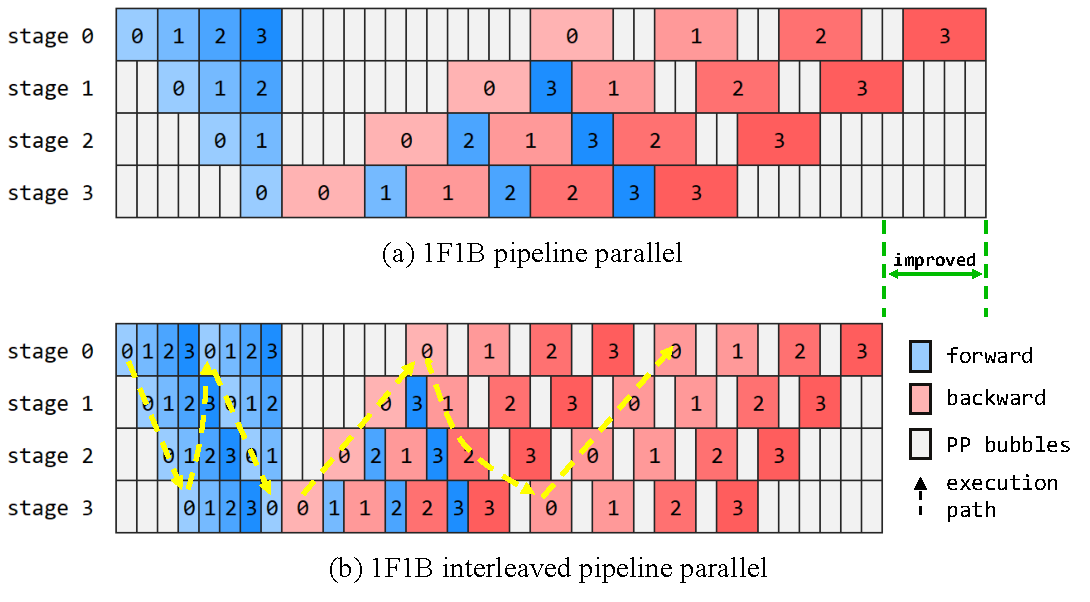
\includegraphics[width=0.8\textwidth]{fig/pipeline_parallelism.pdf}
    \caption{流水并行与交错式流水并行调度示意。}
    \label{fig:interleaved-pp}
\end{figure}

\subsection{系统优化}\label{sec: sys-optimization}

在第~\ref{sec: parallelism} 节 43\% MFU 基线之上，我们进一步加入系统级优化以继续提升训练效率。
通过融合算子、基于子序列切分的上下文并行、数据缓存与共享机制等优化，\modelname~训练效率得到显著提升。
这些优化使系统 MFU 超过 52\%，相较第~\ref{sec: parallelism} 节基线实现约 9\% 相对提升。

\begin{figure}[htbp]
    \centering
    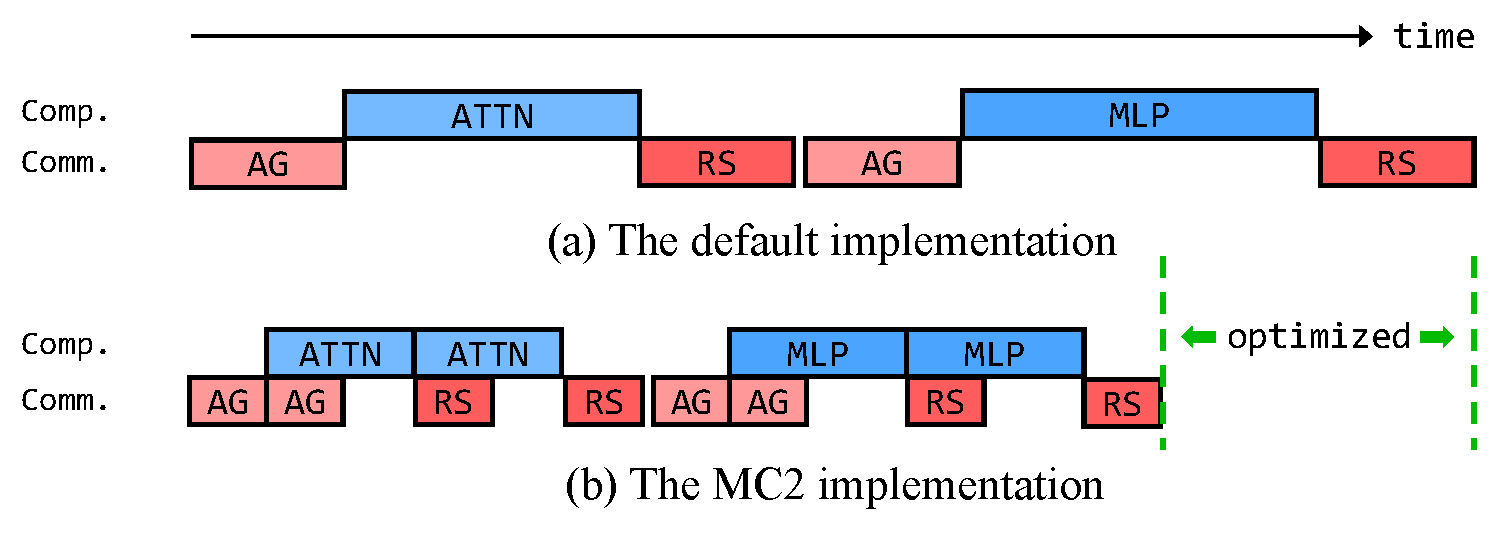
\includegraphics[width=0.7\textwidth]{fig/the_mc2.pdf}
    \caption{默认 Transformer 计算流程与 MC2 方法对比。实际训练中，MC2 会将通信与计算任务融合到单一 kernel。} 
    \label{fig:mc2}
\end{figure}

\subsubsection{Kernel 融合}
Kernel 融合是 LLM 训练中常用的效率优化技术。它将多个操作合并到单个 kernel 中，以减少对全局内存的访问次数~\cite{flash_attention2}。
在 \modelname 训练中，我们对关键算子进行融合，显著提升了硬件利用率和整体训练效率。


\textbf{MC2 - 计算与通信融合（Merged Compute and Communication）}
张量并行结合序列并行时，需要通过 All-Gather（AG）与 Reduce-Scatter（RS）在分布式设备间交换输入/输出激活。
该过程使矩阵乘（MatMul）与 AG/RS 通信存在强依赖关系，从根本上限制了 TP 通信与计算流程的重叠空间。
我们实现了 MC2~\cite{ascend_mc2, mc2} 来解决这一问题，通过将 MatMul 与通信操作融合，缓解该瓶颈。
MC2 将大计算和大通信任务拆分为细粒度子任务，并采用流水化执行以最大化通信与计算重叠。
因此，MC2 显著降低了通信时延并提升硬件利用率（见图~\ref{fig:mc2}）。

\textbf{NPU Fusion Attention}
长序列训练中，自注意力的时间和内存开销会随序列长度增长呈二次增加。
为解决这一问题，Flash Attention（FA）因高性能已成为 LLM 训练标准技术之一~\cite{flash_attention, flash_attention2}。
\modelname~采用专为 Ascend NPU 优化的自注意力融合算子 NPU Fusion Attention（NFA）~\cite{npu_fa}，可在多类自注意力计算场景下带来系统级收益。
\begin{figure}[htbp]
    \centering
    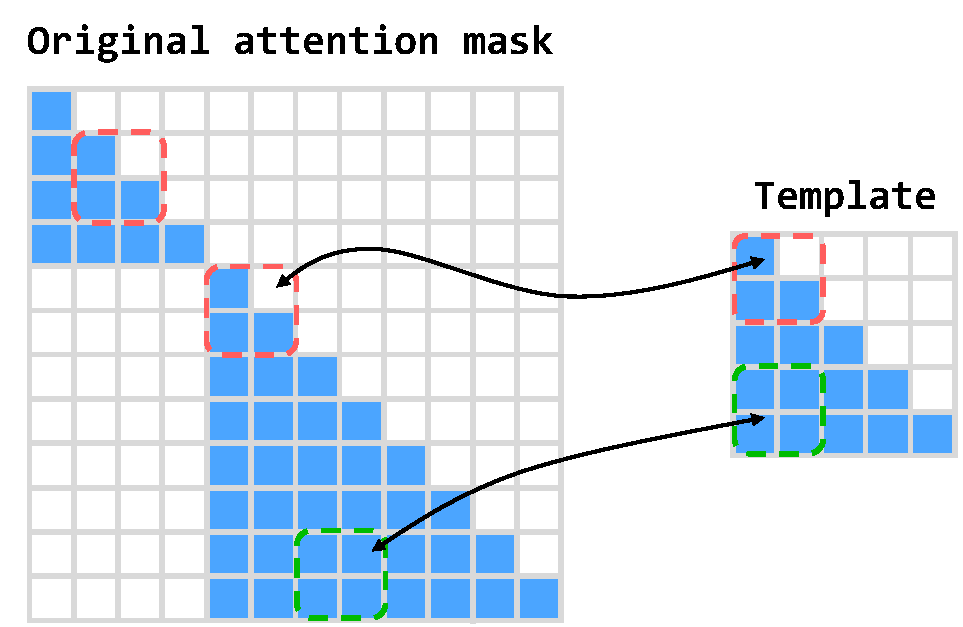
\includegraphics[width=0.4\textwidth]{fig/atten_mask_compression.pdf}
    \caption{NFA 算子中的 attention mask 压缩示例。}
    \label{fig:attn_mask_compression}
\end{figure}

值得一提的是，\modelname~使用 reset attention mask 策略，以阻止同一序列内不同文档间发生自注意力。
这要求为每个序列计算对应 attention mask，带来明显内存和计算开销。
为降低生成 attention mask 的时间与内存成本，NFA 引入了 mask 压缩优化。
如图~\ref{fig:attn_mask_compression} 所示，NFA 使用 $2048 \times 2048$ 因果 mask 作为模板，在融合注意力算子内构造实际计算 mask。
每次迭代时，\modelname~根据文档结束 token（eod）位置获取真实序列长度，并将其作为输入提供给 NFA，以加速自注意力计算。
NFA 的详细使用方式可参见 Ascend 文档~\cite{npu_fa}。

\textbf{其他融合优化}
除 MC2 与 NPU 优化融合注意力外，我们还在 RMSNorm~\cite{zhang2019rootmeansquarelayer}、SwiGLU~\cite{shazeer2020glu}、RoPE~\cite{su2023roformerenhancedtransformerrotary} 等关键模块，以及梯度累积、PP 发送/接收通信等关键流程中引入了系列 kernel 融合优化。
这些融合算子旨在降低 kernel 启动与内存访问开销，同时保持较高数值精度并提升整体训练性能。

\begin{figure}[htbp]
    \centering
    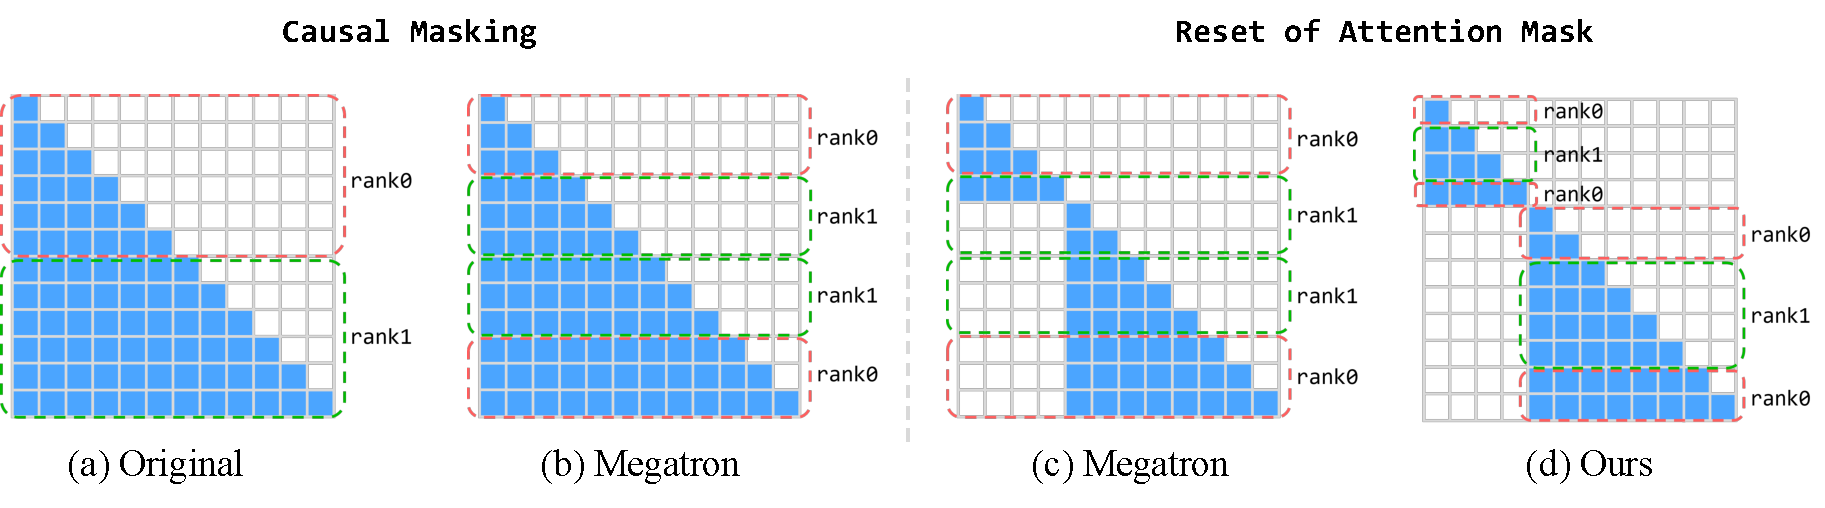
\includegraphics[width=\textwidth]{fig/sub_seq_partition.pdf}
    \caption{用于上下文并行的子序列切分机制示例。}
    \label{fig:sub_seq_partition}
\end{figure}

\subsubsection{长上下文训练优化}
长上下文能力对长文档摘要、对话式 AI 等场景越来越重要。
但长序列训练在时间和内存复杂度上都面临挑战。
为提升长上下文训练效率，我们提出两项关键策略。

\textbf{用于上下文并行的子序列切分}
上下文并行（CP）是训练超长序列的关键方法之一，通过切分输入序列来降低内存消耗~\cite{ringattention, ulysses}。
但在因果 mask 下，若直接将序列切为 $CP$ 份，会导致 Ring Self-Attention（RSA）\cite{ringattention} 负载严重不均衡（图~\ref{fig:sub_seq_partition}(a)）。
Megatron-LM 通过将序列切分为 $2\times CP$ 份来缓解该问题，每个 rank 同时接收顶部和底部的 chunk，从而在 CP 组内平衡负载（图~\ref{fig:sub_seq_partition}(b)）~\cite{megatron-github}。
但在 reset attention mask 场景下，该方法依然存在负载不均衡（图~\ref{fig:sub_seq_partition}(c)）。
因此，在 128K 长上下文训练中，我们提出了更均衡的 CP 切分策略：每个 rank 在每个子序列内负责计算两个 chunk（图~\ref{fig:sub_seq_partition}(d)）。

\textbf{快速 mask 生成与数据复用}
当 \modelname~训练序列长度扩展到 128K 时，attention mask 生成或真实序列长度计算仍会带来不可忽视的性能开销。
另外，在 reset attention mask 的训练场景中，每个 VPP 阶段每次迭代都需获取对应 mask 或真实序列长度，造成重复计算与额外开销。
我们通过两项优化解决该问题：
(1) 使用高效 NPU 算子计算 attention mask，替代 CPU 侧构造方式，从而加速 mask 生成并消除 CPU 与 NPU 间数据传输；
(2) 启用跨 VPP 阶段的 mask 共享机制，由第一阶段（VPP0）生成 attention mask，并在同一 rank 的不同 VPP 阶段共享，避免重复计算和额外内存开销。
